\subsection{Standard Model \ttbar+Z}
\label{sec:Bkg:ttV}

\indent $\ttbar$ produced in conjunction with a $Z$ boson consists of about 1\% of the background in the signal region.  We estimate the amount of $\ttbar+\Zboson$ using a $\ttbar+\gamma$ control region. \\

\indent Using the charged leptonic $Z$ boson decays to design a control region to estimate the $\ttbar+Z$ background would produce a control region with small systematic uncertainty. However, such a control region tends to have low statistics because $Z \rightarrow ee/\mu\mu$ has a lower branching fraction than $Z \rightarrow \nu\nu$.  A dilepton control region also contains a large contribution from SM $\ttbar$ and $Z$ + jets. \\

\indent We take another data driven approach by building a one-lepton control region for $\ttbar+\gamma$.  $\ttbar+\gamma$ mimics $\ttbar+Z$ as the photon is in many ways like a lighter $Z$ boson.  The control region is designed to minimize theoretical uncertainties due to the extrapolation from the $\gamma$ in the control region to the $\Zboson$ in the signal region. \\

\indent We require exactly one {\tt Signal} photon and one {\tt Signal} lepton.  The lepton is not treated as a jet for the purpose of jet multiplicity and jet $\pt$ requirements unlike in the other one lepton control regions.  We also trigger on leptons instead of $\met$ in this region. The lepton triggers used are defined in Table \ref{tb:lepTriggers}.  \\

\begin{table}[h!]
  \begin{center}
    \begin{tabular}{c|c} \hline\hline
      Channel & Trigger \\  \hline
              & {\bf Data 2015} \\ \hline
      Electron & \verb+HLT_e24_lhmedium_L1EM20VH+  \\
      	            & \verb+HLT_e60_lhmedium+ \\
	            & \verb+HLT_e120_lhloose+         \\  
      Muon & \verb+HLT_mu20_iloose_L1MU15+ \\
      	       & \verb+HLT_mu50+ \\
      \hline
              & {\bf Data 2016} \\ \hline
      Electron & \verb+HLT_e26_lhtight_nod0_ivarloose+ \\
                     &\verb+HLT_e60_lhmedium_nod0+ \\
                     &\verb+HLT_e140_lhloose_nod0+         \\ 
      Muon & \verb+HLT_mu26_ivarmedium+ \\ 
                & \verb+HLT_mu50+ \\
      \hline \hline
    \end{tabular}
  \end{center}
  \caption{Single Lepton triggers used in the $\ttbar+\gamma$ control region.  The electron triggers correspond to the a $\pt$ threshold of 24, 26, 60, 120, and 140 $\gev$ respectively.  The muon triggers correspond to $\pt$ thresholds of 20,26 and 50 $\gev$. }
  \label{tb:lepTriggers}
\end{table}

\indent We require the photon $\pt$ be greater than $150\gev$.  The high $\pt$ photon ensures that we are in a region of phase space where the $\gamma$ $\pt$ shape will mimic the heavier $\Zboson$ $\pt$ distribution.  The true $\gamma$ $\pt$ and the $\Zboson$ $\pt$ distributions are shown in Figure \ref{fig:ttZ_vs_ttGamma_pt} after selecting for a boson $\pt$ with greater than $150 \gev$.  We add a systematic uncertainty to account for the difference between the $\gamma$ and $\Zboson$ $\pt$ spectrum. \\

\pagebreak

\begin{figure}[h!]
\centering
\includegraphics[scale=0.4, angle=270]{figures/ttGamma/TruthStudies/Pt150.pdf}
\caption[$\gamma$ and $\Zboson$ $\pT$ distributions in MC simulation with no detector resolution effects]{$\gamma$ and $\Zboson$ $\pT$ distributions in MC simulation with no detector resolution effects.  A selection of $\pt > 150 \gev$ has been applied.}
\label{fig:ttZ_vs_ttGamma_pt}
\end{figure}

\indent The $\ttbar+\gamma$ control region is defined in Table~\ref{tb:ttG_1lepSel}.  The expected background and data yields in the $\ttbar+\gamma$ control region is given in Table \ref{table.bkgonly.CRTTgamma}. \\

\begin{table}[h!]
  \begin{center}
    \begin{tabular}{c|c}
      \hline \hline
      Selection                 & Requirement     \\
      \hline \hline
      Event selection & Event cleaning \\
      \hline
       Trigger  & 1L Triggers  \\  \hline
      Leptons & $= 1$ \\
      Lepton \pt & 28 $\GeV$ \\
      \hline
      Photons & exactly 1\\
      \hline
      jet multiplicity & $ \ge 4 $ \\
      \hline
      Jet \pT\ & (80,80,40,40) GeV \\
      \hline
      b-jet multiplicity & $\ge 2$ \\
      \hline
      $\gamma$ \pT\ & $> 150$ GeV \\
      \hline\hline
    \end{tabular}
  \end{center}
    \caption[Selections for the $\ttbar+\gamma$ one lepton control region]{Selections for the $\ttbar+\gamma$ one lepton control region. The one lepton triggers as described in Table~\ref{tb:lepTriggers}}
      \label{tb:ttG_1lepSel}
\end{table}




\begin{table}[!h]
\begin{center}
\setlength{\tabcolsep}{0.0pc}
{\small
%%
\begin{tabular*}{\textwidth}{@{\extracolsep{\fill}}lr}
\noalign{\smallskip}\hline\noalign{\smallskip}
{\bf CRTTgamma yields}           & CRTTGamma              \\[-0.05cm]
\noalign{\smallskip}\hline\noalign{\smallskip}
%%
Observed events          & $161$                    \\
\noalign{\smallskip}\hline\noalign{\smallskip}
%%
Fitted bkg events         & $161.19 \pm 14.03$              \\
\noalign{\smallskip}\hline\noalign{\smallskip}
%%
        Fitted TTbar events         & $4.75_{-4.75}^{+9.52}$              \\
%%
        Fitted Wjets events         & $0.05 \pm 0.01$              \\
%%
        Fitted Zjets events         & $0.75 \pm 0.19$              \\
%%
        Fitted TtbarV events         & $3.01 \pm 0.42$              \\
%%
        Fitted TtbarGamma events         & $143.96 \pm 13.37$              \\
%%
        Fitted SingleTop events         & $2.40 \pm 0.84$              \\
%%
        Fitted Diboson events         & $0.00 \pm 0.00$              \\
%%
        Fitted VGamma events         & $6.27 \pm 1.63$              \\
%%     
 \noalign{\smallskip}\hline\noalign{\smallskip}
%%
MC exp. SM events              & $128.31 \pm 18.89$              \\
\noalign{\smallskip}\hline\noalign{\smallskip}
%%
        MC exp. TTbar events         & $5.14_{-5.14}^{+11.21}$              \\
%%
        MC exp. Wjets events         & $0.04 \pm 0.01$              \\
%%
        MC exp. Zjets events         & $0.66 \pm 0.13$              \\
%%
        MC exp. TtbarV events         & $2.34 \pm 0.37$              \\
%%
        MC exp. TtbarGamma events         & $111.77 \pm 13.41$              \\
%%
        MC exp. SingleTop events         & $2.07 \pm 0.40$              \\
%%
        MC exp. Diboson events         & $0.00 \pm 0.00$              \\
%%
        MC exp. VGamma events         & $6.29 \pm 1.64$              \\
%%     \\
\noalign{\smallskip}\hline\noalign{\smallskip}
Fitted $\ttbar+\gamma$ normalization scale factor & $1.29 \pm 0.20$ \\
\noalign{\smallskip}\hline\noalign{\smallskip}
\end{tabular*}
%%%
}
\end{center}
\caption[$\ttbar+\gamma$ control region MC Yield and background-only fit results for $\intlumi$ $\ifb$ of data]{$\ttbar+\gamma$ control region MC Yield and background-only fit results for $\intlumi$ $\ifb$ of data. MC exp. events are expected background rates directly from MC predictions.  Fitted background event rates are the expected background rates after normalizing the MC to data by simultaneously fitting all control regions using a background-only fit.  The fitted $\ttbar+\gamma$ normalization scale factor is equal to (Fitted $\ttbar+\gamma$ events)/(MC exp. $\ttbar+\gamma$ events). The quoted uncertainties include statistical and systematic uncertainties. }
\label{table.bkgonly.CRTTgamma}
\end{table}
%

\indent Kinematic distributions in the $\ttbar+\gamma$ control region are shown in Figure ~\ref{fig:ttgamma}  The MC background has been normalized to data by performing a simultaneous fit to all the control regions.  The hashed bands on the total SM background correspond to the total experimental systematical uncertainty plus the MC statistical uncertainty.   \\

\pagebreak

\begin{figure}[h!]
\begin{center}
      \begin{subfigure}[b]{0.40\textwidth}    
\includegraphics[width=\textwidth]{figures/ttGamma/Met_CRTTGamma_withRatio_log.eps}
                 \caption{ }
    \end{subfigure}
      \begin{subfigure}[b]{0.40\textwidth}    
      \includegraphics[width=\textwidth]{figures/ttGamma/postfit/NJets_CRTTGamma_log.eps}
                 \caption{ }
    \end{subfigure}
      \begin{subfigure}[b]{0.40\textwidth}    
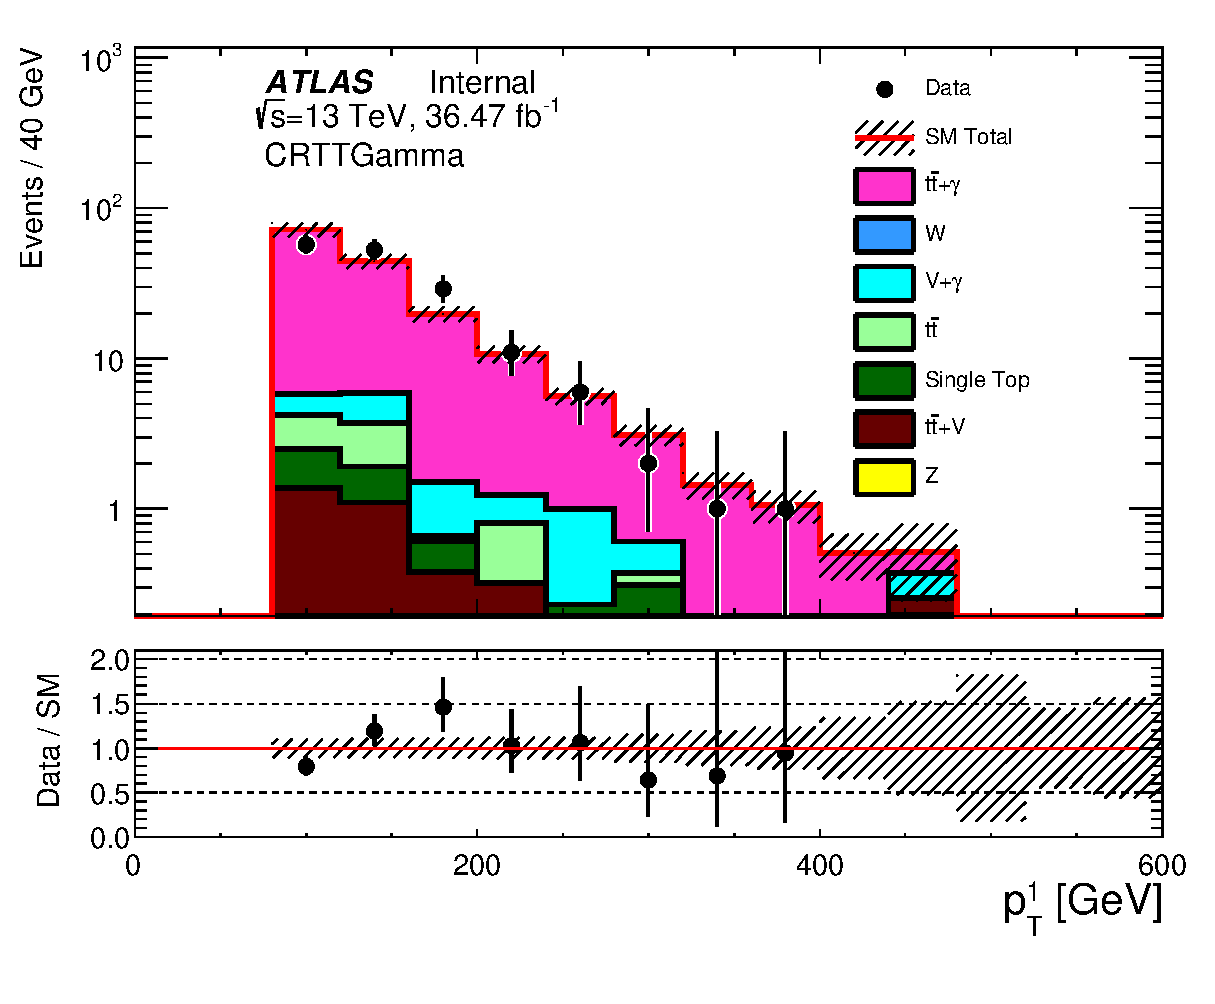
\includegraphics[width=\textwidth]{figures/ttGamma/postfit/JetPt_1__CRTTGamma_log.eps}
                 \caption{ }
    \end{subfigure}
      \begin{subfigure}[b]{0.40\textwidth}    
\includegraphics[width=\textwidth]{figures/ttGamma/postfit/JetPt_4__CRTTGamma_log.eps}
                 \caption{ }
    \end{subfigure}
%      \begin{subfigure}[b]{0.40\textwidth}    
%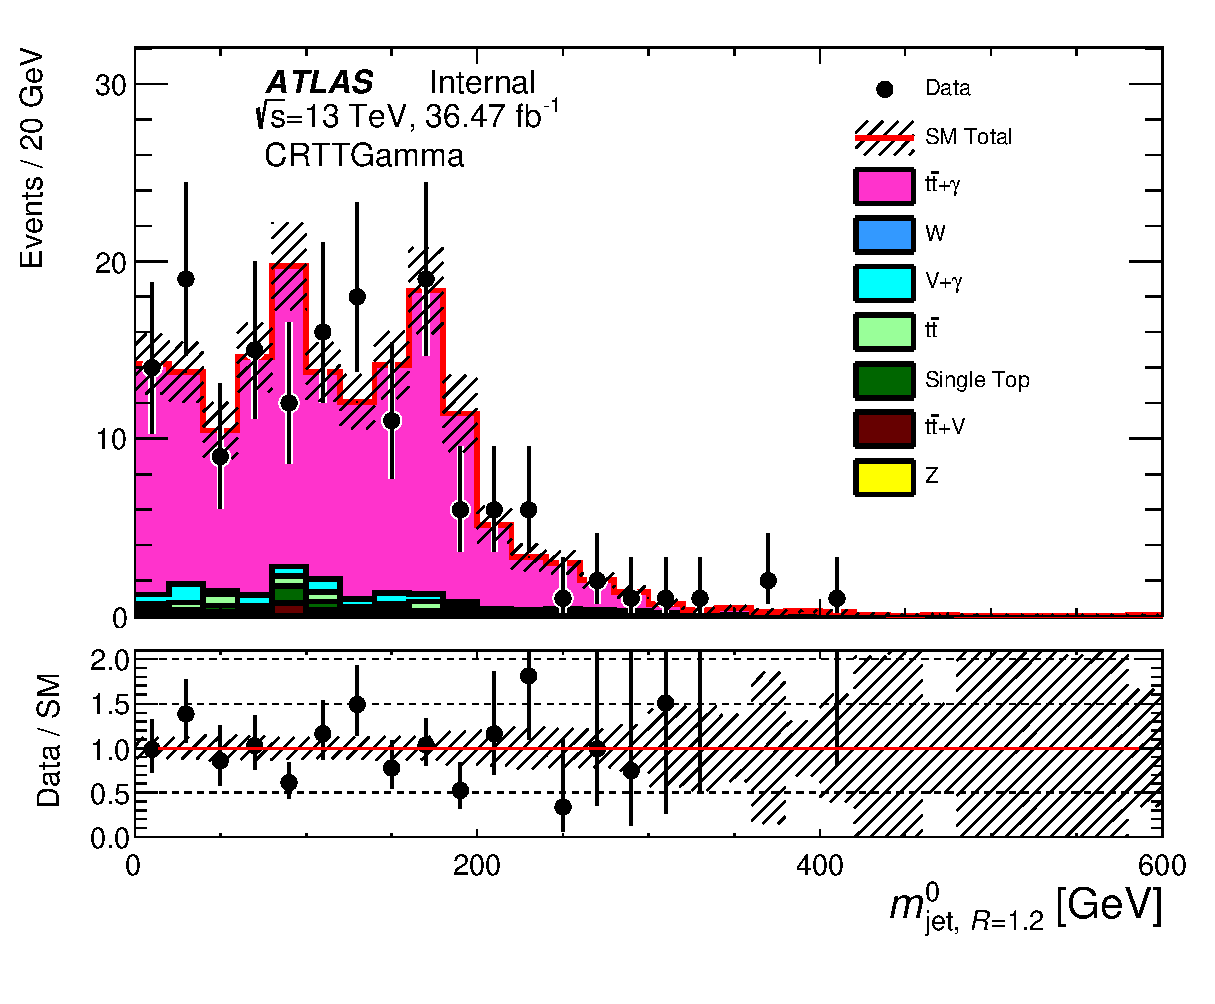
\includegraphics[width=\textwidth]{figures/ttGamma/postfit/AntiKt12M_0__CRTTGamma.eps}
%                 \caption{ }
%    \end{subfigure}
%      \begin{subfigure}[b]{0.40\textwidth}    
%\includegraphics[width=\textwidth]{figures/ttGamma/MtMetLep_CRTTGamma_withRatio_log.eps}
%                 \caption{ }
%    \end{subfigure}
\caption[Distributions of select kinematic variables in the $\ttbar+\gamma$ control region]{ Distributions of select kinematic variables in the $\ttbar+\gamma$ control region. Kinematic variables shown include (a) $\met$ (b) number of jets (c) $\pt$ of the 2nd highest $\pt$ jet (d) $\pt$ of the 5th highest $\pt$ jet. The hashed area in both the top and lower panel represents the uncertainty due to MC statistics.}
\label{fig:ttgamma}
\end{center}
\end{figure}





